\documentclass[12pt]{article}

\usepackage{algorithm}
\usepackage[noend]{algpseudocode}
\usepackage{amssymb,amsmath,amsthm,multirow, graphicx, amsfonts,latexsym,mathtext, array, enumerate, verbatim, hyperref, listings,color,geometry, caption, subcaption, dsfont}

\newtheorem{cor}{Corollary}
\newtheorem{thm}{Theorem} 
\newtheorem{lem}{Lemma}
\newtheorem{prop}{Proposition}
\newtheorem{mydef}{Definition}
\newtheorem{rem}{Remark}
\newcommand{\M}{\mathbf}
\newcommand{\MS}{\boldsymbol}
\newcommand{\Cal}{\mathcal}
\newcommand{\U}{\mathcal{U}}
\newcommand{\R}{\mathbb{R}}
\newcommand{\1}{\mathds{1}}
\newcommand{\dx}{\Delta x}
\newcommand{\dy}{\Delta y}


\newenvironment{claim}[1]{\par\noindent\underline{Claim:}\space#1}{}
\newenvironment{claimproof}[1]{\par\noindent\underline{Proof:}\space#1}{\hfill $\blacksquare$}


\begin{document}

\title{15.097 - Homework 1}
 
\author{Colin Pawlowski}
\maketitle

\section{Compressed Sensing}
Assume $\M A$ is an $m \times n$ matrix, $n > m$.  Consider the problem
\begin{equation}
\begin{array}{rll}
  \min & \|\M x\|_0 \vspace{5pt}\\
  \text{s.t.} & \M{Ax = b}.
\end{array}
\end{equation}\\
%
Using MIO, we reformulate this problem as
\begin{equation}
\label{eq1:MIO}
\begin{array}{rll}
  \min & \sum \limits_{i=1}^n z_i \vspace{5pt}\\
  \text{s.t.} & \M{Ax = b},  \vspace{3pt}\\
  & -Mz_i \le x_i \le Mz_i &~~~i=1,\ldots,n, \vspace{3pt}\\
  & z_i \in \{0,1\} &~~~i=1,\ldots,n. \vspace{3pt}\\
\end{array}
\end{equation}\\
%
Next, consider the problem
\begin{equation}
\begin{array}{rll}
  \min & \|\M x\|_1 \vspace{5pt}\\
  \text{s.t.} & \M{Ax = b}.
\end{array}
\end{equation}\\
%
Using linear optimization, we can reformulate this problem as
\begin{equation}
\label{eq1:LO}
\begin{array}{rll}
  \min & \sum \limits_{i=1}^n y_i \vspace{5pt}\\
  \text{s.t.} & \M{Ax = b},  \vspace{3pt}\\
  & -y_i \le x_i \le y_i &~~~i=1,\ldots,n. \vspace{3pt}\\
\end{array}
\end{equation}\\

We implemented both optimization problems~\ref{eq1:MIO} and \ref{eq1:LO} in JuMP.  For the simulated experiments, we generated a random $20 \times 20$ matrix $\M M$ with entries $a_{ij} \sim N(0,1)~i.i.d.$.  For a fixed triplet $(k, m, n)$, we solved problems~\ref{eq1:MIO} and \ref{eq1:LO}, where $\M A$ is the upper $m \times n$ submatrix of $\M M$, $\M{x_0} \in \{0,1\}^n$ is the vector with the first $k$ components 1 and the rest 0, and $\M{b = Ax_0}$.   We repeated this experiment for all possible combinations $k \le m \le n = 20$, and tracked the number of successfully recovered components of $\M x_0$ recovered by each method.  

We found that the MIO formulation always found a solution with at most $k$ nonzero components, and in some cases found solutions which were even more sparse than $\M{x_0}$ due to numerical approximations.  On the other hand, the LO formulation correctly recovered the $\M{x_0}$ solution sometimes, but in many cases LO yielded solutions with greater than $k$ nonzero components.  We plot the results in phase diagrams with axes $m/n$ and $k/m$, indicating whether or not the correct sparsity pattern was recovered at each data point.  

\begin{figure}[tb]
  \centering
  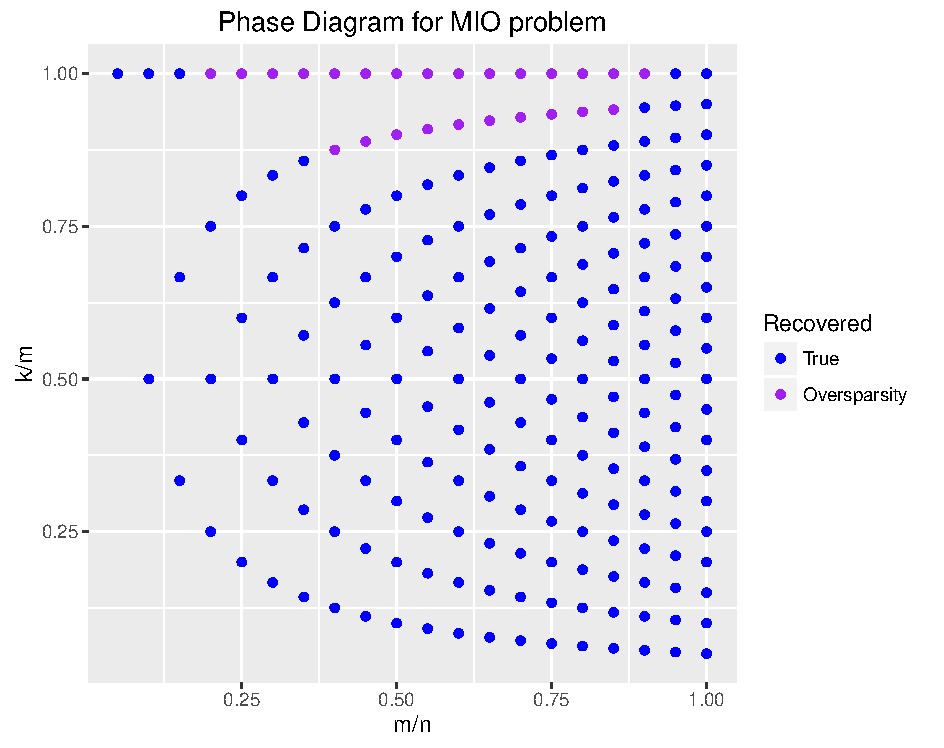
\includegraphics[width=0.8\textwidth]{phase_MIO}
  \caption{Phase diagram for MIO.}\label{fig:MIO_phase}
\end{figure}

\begin{figure}[tb]
  \centering
  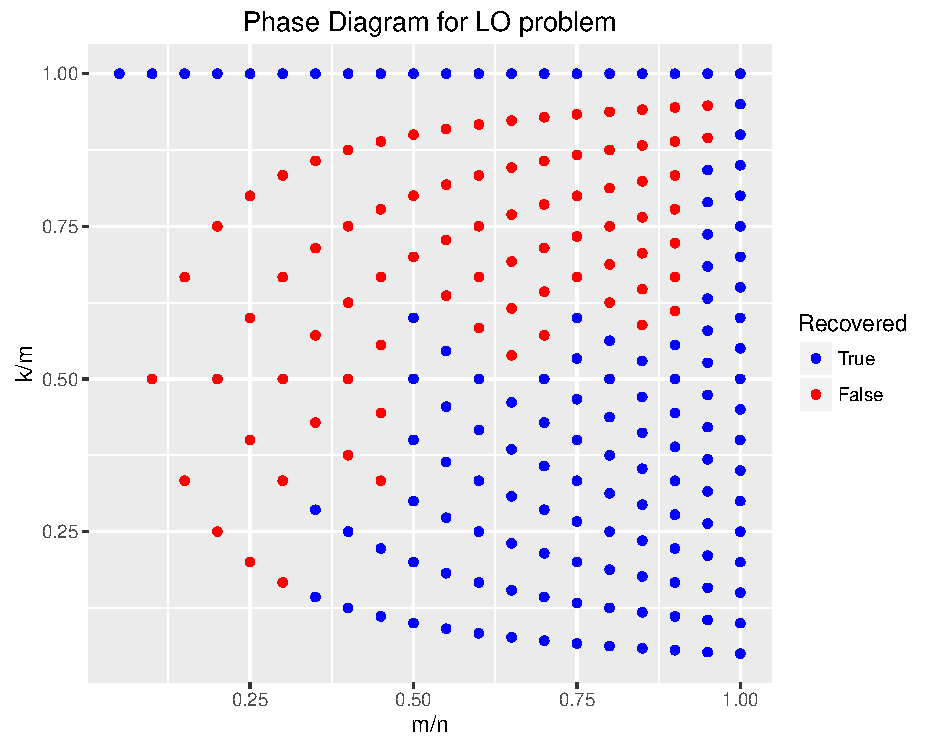
\includegraphics[width=0.8\textwidth]{phase_LO}
  \caption{Phase diagram for LO.}\label{fig:LO_phase}
\end{figure}

\section{Algorithmic Framework for Regression using MIO}

We implemented an algorithmic framework for regression in JuMP, building upon the code BestSubset.jl which already incorporates sparsity.  To incorporate robustness, we added an L-0 penalty term $\Gamma \|\MS \beta\|_1$ to the objective and used cross-validation to find the optimal value of robustness parameter $\Gamma$. Searching over the range $\Gamma \in \{10^{-6},10^{-5},\ldots,10^2\}$, we found that the optimal value $\Gamma = 0.01$.  To incorporate pairwise collinearity, we computed the complete correlation matrix and added a threshold input $\rho_{max}$ specified by the user.  For all features $(\beta_i, \beta_j)$ with pairwise correlation $\rho_{ij} > \rho_{max}$, we added the constraint $z_i + z_j \le 1$.  To incorporate group sparsity, we added user input a list of subsets $S_1,\ldots, S_k \subset \{1,\ldots, D\}$.  For each group $g = 1,\ldots,k$, we add the constraints $z_i = z_j, \forall i,j \in S_k$.  To incorporate nonlinear transformations, we appended the features $\sqrt{\beta_i}, \beta_i^2, \log \beta_i$ to the training, validation, and test matrices for all features $\beta_i, i=1,\ldots,D$.  We then ran the MIO problem with the full feature vector $\hat{\MS \beta} = [\beta_1,\ldots, \beta_D, \sqrt{\beta_1}, \ldots, \sqrt{\beta_D}, \beta_1^2, \ldots, \beta_D^2, \log \beta_1, \ldots, \log \beta_D]$.   To ensure that only one transformation of each feature would be used in the final model, we added the constraints $z_i + z_{i+D} + z_{i+2D} + z_{i+3D} \le 1$ for all $i = 1,\ldots,D$.    Finally, we added a user input boolean to check for statistical significance.  If true, then each time we find a model with improved validation set $R^2$, we compute the standard linear regression on the features that have nonzero $\beta_i$ coefficients in the current solution.  If one or more of the independent variables in this regression are not statistically significant, then we do not update the current best solution, and we add a constraint to exclude this particular solution from the MIO feasible region.  Assume that we find solution $\MS {\tilde \beta}$ that is not statistically significant, with associated sparsity vector $\M {\tilde z} \in \{0,1\}^D$.  To exclude this solution for the next MIO solve, we add the constraint
\[
\sum_{i=1}^D {\tilde z_i} z_i + (1 - {\tilde z_i})(1 - z_i) \le D - 1.
\]

Running our model with sparsity, nonlinear transformations, and maximum pairwise correlation 0.8, we obtain a model with maximum pairwise correlation 0.784, sparsity $K = 7$ nonzero coefficients including features $[\beta_{10}, \beta_{12}, \beta_{13}, \beta_{18}, \beta_{22}, \beta_{37}, \beta_{38}]$, which yields Out-of-Sample $R^2 = 0.815$ in 11.437 seconds.  Running our model with sparsity, robustness, statistical significance, and maximum pairwise correlation 0.8, we obtain a model with maximum pairwise correlation 0.784, robustness parameter $\rho = 0.0$, sparsity $K = 3$ nonzero coefficients including features $[\beta_{7}, \beta_{10}, \beta_{11}]$, which yields Out-of-Sample $R^2 = 0.806$ in 0.553 seconds.


\section{First Order Method}

Here, we derive a first order method following the notes from Lecture 2 - Best Subset Selection.  Consider the problem
\begin{equation}
\begin{array}{rll}
  \min \limits_{\MS \beta} & g(\MS \beta) := \|\M y - \M X \MS \beta \|_2^2 + \Gamma \| \MS \beta \|_1 \vspace{5pt}\\
  \text{s.t.} & \| \MS \beta \|_0 \le k.
\end{array}
\end{equation}\\

Since $g(\MS \beta)$ is convex and $\|\nabla g(\MS \beta) - \nabla g(\MS \beta_0)\| \le \ell \| \MS \beta - \MS \beta_0\|$, it follows that for all $L \ge \ell$

\begin{equation}
g(\MS \beta) \le Q(\MS \beta) := g(\MS \beta_0) + \nabla g(\MS \beta_0)^T(\MS \beta - \MS \beta_0) + \frac{L}{2} \|\MS \beta - \MS \beta_0\|_2^2 + \Gamma \| \MS \beta \|_1.
\end{equation}\\

To find feasible solutions, we solve the following problem
\begin{equation}
\begin{array}{rll}
  \min \limits_{\MS \beta} & Q(\MS \beta) \vspace{5pt}\\
  \text{s.t.} & \| \MS \beta \|_0 \le k.
\end{array}
\end{equation}\\

This is equivalent to
\begin{equation}
\begin{array}{rll}
  \min \limits_{\MS \beta} & \displaystyle \frac{L}{2}\Big\|\MS \beta - \Big(\MS \beta_0 - \frac{1}{L} \nabla g(\MS \beta_0)\Big) \Big\|_2^2 - \frac{1}{2L} \|\nabla g(\MS \beta_0) \|_2^2 + \Gamma \| \MS \beta \|_1 \vspace{5pt}\\
  \text{s.t.} & \| \MS \beta \|_0 \le k,
\end{array}
\end{equation}\\

which reduces to the following plus a constant term:
\begin{equation}
\label{u_prob}
\begin{array}{rll}
  \min \limits_{\MS \beta} & \displaystyle \frac{L}{2}\|\MS \beta - \M u \|_2^2 + \Gamma \| \MS \beta \|_1 \vspace{5pt}\\
  \text{s.t.} & \| \MS \beta \|_0 \le k.
\end{array}
\end{equation}\\

For the vector $\M u \in \R^p$, let $(1), (2), \ldots (p)$ be the indices of the order statistics $|u_{(1)}| \ge |u_{(2)}| \ge \ldots \ge |u_{(p)}|$.  At the optimal solution $\MS \beta^*$ to problem~\ref{u_prob}, we have $|\beta_{(1)}^*| \ge |\beta_{(2)}^*| \ge \ldots \ge |\beta_{(p)}^*|$, which implies that $|\beta_{(k+1)}^*| = |\beta_{(k + 2)}^*| = \ldots = |\beta_{(p)}^*| = 0$.  For $i \le k$, $\beta_{(i)}^*$ is the optimal solution to the following unconstrained single variable problem:

\begin{equation}
\label{eq:1var}
\min \limits_{\beta_{(i)}} \frac{L}{2}(\beta_{(i)} - u_{(i)})^2 + \Gamma |\beta_{(i)} |.
\end{equation}\\

Problem~\ref{eq:1var} has closed form solution

\begin{equation}
\beta_{(i)}^* = \left\{\begin{array}{rl} 
u_{(i)} - \displaystyle \frac{\Gamma}{L}\text{sign}(u_{(i)}), &~~~{\rm if}~|u_{(i)}| \ge \displaystyle \frac{\Gamma}{L}, \vspace{5pt}\\
0, &~~~\rm{otherwise.}
\end{array} \right.
\end{equation}\\

Thus, the optimal solution to problem~\ref{u_prob} is $\MS \beta^* = \M H_k(\M u)$, where
\begin{equation}
(\M H_k(\M u))_i = \left\{\begin{array}{rl} 
u_{(i)} - \displaystyle \frac{\Gamma}{L}\text{sign}(u_{(i)}), &~~~{\rm if}~|u_{(i)}| \ge \displaystyle \frac{\Gamma}{L}~{\rm and}~i \le k, \vspace{5pt}\\
0, &~~~\rm{otherwise.}
\end{array} \right.
\end{equation}

Using this update iteratively to determine the $\beta_i$'s, we obtain the following first order method:\\

\underline{\bf Algorithm 1}\\

\emph{Input}: $g(\MS \beta), L, \epsilon$.\\

\emph{Output}: A first order stationary solution $\MS \beta^*$.

\begin{enumerate}
	\item Initialize with $\MS \beta_1 \in \R^p$ such that $\|\MS \beta_1\|_0 \le k$.
	\item For $m \ge 1$
	\[
	\MS \beta_{m+1} \leftarrow \M H_k(\MS \beta_0 - \frac{1}{L} \nabla g(\MS \beta_0))
	\]
	\item Repeat Step 2, until $g(\MS \beta_m) - g(\MS \beta_{m+1}) \le \epsilon$.
\end{enumerate}

\end{document}
